\subsection{Gerichtete Graphen}
\begin{frame}{Gerichtete Graphen}
	\begin{block}{Def.: Gerichteter Graph}
		Ein \textbf{gerichteter Graph} $G$ ist ein Paar $G=(V,E)$.
		\begin{itemize}
			\item $V$ heißt \textbf{Knotenmenge}.
				\begin{itemize}
					\item Knoten haben Bezeichner (entspricht Beschriftung), z.B. $V=\set{a,b,c,...}, V=\set{1,2,3,...}, V=\set{start, z1, z2, end}, ...$
				\end{itemize}
			\item $E \subseteq V \times V$ heißt \textbf{Kantenmenge}.
				\begin{itemize}
					\item Kanten sind also Paare aus Knoten in $V$, z.B. $E=\set{(a,b),\; (b,c)}, ...$
					\item $(x,y) \in E \Rightarrow$ Es gibt eine Kante vom Knoten $x$ zum Knoten $y$.
				\end{itemize}
		\end{itemize}
	\end{block}
\end{frame}

\begin{frame}{Gerichtete Graphen}

	\begin{exampleblock}{Beispiel}
		\begin{figure}[H]
		\begin{tikzpicture}[->,>=stealth,baseline=-5mm]
		\matrix[matrix of math nodes,nodes={draw,circle,minimum size=10mm,inner sep=2pt},row sep=15mm,column sep=15mm,ampersand replacement=\&]
		{
			|(1)| 1 \& |(5)| 5 \& |(3)| 3 \\
			|(0)| 0 \& |(2)| 2 \& |(4)| 4 \\
		};
		\draw  (0) to [bend left] (1);
		\draw  (1) to [bend left] (0);
		\draw  (1) -- (2);
		
		\draw  (4) -- (5);
		\draw  (4) to [bend left] (3);
		\draw  (3) to [bend left] (4);
		\end{tikzpicture}
		\end{figure}

	Graph definiert durch $G = (V, E)$ mit $V = \{0,1,2,3,4,5\}$ und $E = \{(0,1), (1,0), (1,2), (3,4), (4,3) ,(4,5)\}$.
	\end{exampleblock}
\end{frame}

\begin{frame}{Aufgabe: Gerichtete Graphen zeichnen}
	\begin{exampleblock}{Aufgabe}
		Zeichnet die Graphen $G_i = (V, E_i)$ mit $V = \nZ_4$ und
		\begin{enumerate}
			\item $E_1 = \{(0,1), (0,2), (0,3), (1,2), (1,3), (2,2), (2,3), (3,2)\}$
			\item $E_2 = \{(0,1), (0,2), (0,3) \}$
			\item $E_3 = \emptyset$
			\item $E_4 = V \times V$
			\item $E_5 = \{(0,1), (1,2), (1,3)\}$
		\end{enumerate}
	\end{exampleblock}
	
\end{frame}

\begin{frame}{Gerichtete Graphen: Pfade}
	\begin{block}{Def.: Pfad}
		Sei $G=(V,E)$ ein gerichteter Graph. Ein $(n+1)$-Tupel $p=(v_0,v_1,...,v_n)$ mit $v_i \in V \; (i \in \set{0,...,n})$ heißt \textbf{Pfad von $v_0$ nach $v_n$ der Länge $n$}, gdw. \\
		\[
			\forall i \in \set{0, ..., n-1}: (v_i, v_{i+1}) \in E
		\]
		\\[12pt]
		Die Länge des Pfades ist also gleich der Anzahl der Kanten (!).

		Länge 0 für Pfade erlaubt: $p = (v_0)$
	\end{block}

	\begin{exampleblock}{Beispiele}
		Auf Graph oben existieren z.B. Pfade $p_1=(3,4,5)$ oder $p_2=(1,0,1,2)$.
	\end{exampleblock}
\end{frame}

\begin{frame}{Aufgabe: Pfade erkennen}
	\begin{exampleblock}{Aufgabe}
	\begin{center}
		
	\begin{columns}
		\begin{column}{0.475\textwidth}
			$G_1:$
			\begin{figure}[H]
			\begin{tikzpicture}[->,>=stealth,baseline=-5mm]
				\matrix[matrix of math nodes,nodes={draw,circle,minimum size=8mm,inner sep=2pt},row sep=10mm,column sep=10mm,ampersand replacement=\&]
				{
				    		\& |(4)| 4 \\
					|(0)| 0 \& |(1)| 1 \\
					|(2)| 2 \& |(3)| 3 \\
				};
				\draw  (0) -- (2);
				\draw  (3) -- (2);
				\draw  (1) -- (3);
				\draw  (4) -- (1);
			\end{tikzpicture}
			\end{figure}
		\end{column}
		\begin{column}{0.475\textwidth}
			$G_2:$
			\begin{figure}[H]
			\begin{tikzpicture}[->,>=stealth,baseline=-5mm]
				\matrix[matrix of math nodes,nodes={draw,circle,minimum size=8mm,inner sep=2pt},row sep=10mm,column sep=10mm,ampersand replacement=\&]
				{
					|(0)| 0 \& |(1)| 1 \\
					|(2)| 2 \& |(3)| 3 \\
				};
				\draw  (0) -- (2);
				\draw  (3) -- (2);
				\draw  (1) -- (3);
				\draw  (2) -- (1);
			\end{tikzpicture}
			\end{figure}
		\end{column}
	\end{columns}
	\end{center}
	Gib alle Pfade auf $G_1$ und $G_2$ an.

	\end{exampleblock}
\end{frame}
	
\begin{frame}
	\begin{block}{Lösung}
	\begin{itemize}
		\item Pfade auf $G_1$: \begin{itemize}
			\item $p_1=(4,1), \; p_2=(1,3), \; p_3=(3,2), \; p_4=(0,2)$,
			\item $p_5=(4,1,3), \; p_6=(1,3,2)$,
			\item $p_7=(4,1,3,2)$
			\end{itemize}
		\item Pfade auf $G_2$: ???
	\end{itemize}
	\end{block}
		
	Warum können wir die Pfade auf $G_2$ nicht angeben?\newline
	\pause

	$G_2$ enthält einen \textbf{Zyklus}...

\end{frame}

\begin{frame}{Gerichtete Graphen: Zyklen}
	\begin{block}{Def.: Zyklus}
		Ein Pfad $p=(v_0,...,v_n)$ mit $v_0=v_n$ heißt \textbf{geschlossen}.
		\begin{itemize}
			\item Ein geschlossener Pfad mit $n \ge 1$ heißt \textbf{Zyklus}.
			\item Enthält ein Graph keine Zyklen, so heißt er \textbf{azyklisch} (DAG).
		\end{itemize}		
	\end{block}
	\pause
	\begin{block}{Def.: Wiederholungsfreiheit}
		Ein Pfad $p=(v_0,...,v_n)$ heißt \textbf{wiederholungsfrei}, gdw. 
		\begin{itemize}
			\item $v_0,...,v_{n-1}$ und $v_1,...,v_n$ jeweils paarweise verschieden sind.
			\item D.h. alle Knoten müssen sich unterscheiden, nur $v_0$ und $v_n$ dürfen gleich sein.
		\end{itemize}
		\medskip
		Ein \textbf{einfacher Zyklus} ist ein wiederholungsfreier Zyklus.
	\end{block}
	
\end{frame}
		
\begin{frame}{Aufgabe: Graphen konstruieren}
	\begin{exampleblock}{Aufgabe}
		Finde einen Graphen $G=(V,E)$, der die folgenden Eigenschaften hat:
		\begin{itemize}
		 	\item G ist streng zusammenhängend\footnote{$G=(V,E)$ streng zusammenhängend $:\Leftrightarrow$ $\forall u,v \in V: \exists$ Pfad von $u$ nach $v$}.
		 	\item G hat mindestens zwei unterschiedliche Zyklen, die sich nicht nur durch beliebig häufige Wiederholungen unterscheiden.\\
		 	Das bedeutet, $p=(0,1,0) \neq q=(0,1,0,1,0)$ reicht nicht.
		 	\item G hat mindestens einen einfachen Zyklus.
		 \end{itemize}
		 \medskip
		 Gib die Mengen $V$ und $E$ an und zeichne den Graphen G.
	\end{exampleblock}
\end{frame}
	
\begin{frame}{Aufgabe: Graphen konstruieren}
	\begin{block}{Lösung}
		Eine mögliche Lösung ist $G=(V,E)$ mit $V=\set{1,2}$ und $E=\set{(1,2) \; (2,1) \; (1,1)}$. \\[18pt]
		$G:$

		\begin{center}
		\begin{figure}[H]
			\begin{tikzpicture}[->,>=stealth,baseline=-5mm]
				\matrix[matrix of math nodes,nodes={draw,circle,minimum size=8mm,inner sep=2pt},row sep=10mm,column sep=10mm,ampersand replacement=\&]
				{
					|(1)| 1 \& \\
					|(2)| 2 \& \\
				};
				\draw  (1) to [bend left] (2);
				\draw  (2) to [bend left] (1);
				\path  (1) edge [loop above] ();
			\end{tikzpicture}
			\end{figure}
		\end{center}
	\end{block}
\end{frame}

\begin{frame}{Gerichtete Graphen: Knotengrad}
	\begin{block}{Def.: Knotengrade}
		Sei $G=(V,E)$ ein gerichteter Graph und $v \in V$.
		\begin{itemize}
			\item \textbf{Eingangsgrad von $v$}: Anzahl eingehender Kanten, $d^{-}(v) = \setsize{\setc{x}{(x,v)\in E}}$
			\item \textbf{Ausgangsgrad von $v$}: Anzahl ausgehender Kanten, $d^{+}(v) = \setsize{\setc{x}{(v,x)\in E}}$
			\item \textbf{Grad von $v$}: $d(v) = d^{+} + d^{-}$
		\end{itemize}
	\end{block}
\end{frame}

\begin{frame}{Gerichtete Graphen: Gerichtete Bäume}
	\begin{block}{Def.: Baum}
		Ein gerichteter Graph $G=(V,E)$ heißt \textbf{gerichteter Baum}, gdw. es eine \textbf{Wurzel} $r \in V$ gibt, von der aus es genau einen Pfad zu jedem Knoten gibt.\\
		Oder Formell: $\exists r \in V: \forall x \in V: \exists_1 Pfad \; p=(r,...,x) $
	\end{block}

	\begin{exampleblock}{Beispiel}
		Ein Ableitungsbaum einer kontextfreien Grammatik ist ein gerichteter Baum mit dem Startsymbol als Wurzel.
	\end{exampleblock}
\end{frame}

\begin{frame}{Gerichtete Graphen: Gerichtete Bäume}
	\begin{center}
		\begin{figure}[H]
			\begin{tikzpicture}[->,>=stealth,baseline=-5mm]
				\matrix[matrix of math nodes,nodes={draw,circle,minimum size=8mm,inner sep=2pt},row sep=10mm,column sep=10mm,ampersand replacement=\&]
				{
					        \& |(1)| 1 \& 		  \&		\\
					|(2)| 2 \& |(3)| 3 \& |(4)| 4 \&		\\
					|(5)| 5 \& |(6)| 6 \& |(7)| 7 \& |(8)| 8\\
				};
				\draw  (1) -- (2);
				\draw  (1) -- (3);
				\draw  (1) -- (4);
				\draw  (2) -- (5);
				\draw  (2) -- (6);
				\draw  (4) -- (7);
				\draw  (4) -- (8);
			\end{tikzpicture}
		\end{figure}
	\end{center}

		Wir nennen in einem gerichteten Baum die Knoten mit Ausgangsgrad = 0 \textbf{Blätter} (hier: $3,5,6,7,8$).\\
		Wir nennen in einem gerichteten Baum die Knoten mit Ausgangsgrad > 0 \textbf{innere Knoten} (hier: $1,2,4$).

\end{frame}

\subsection{Ungerichtete Graphen}

\begin{frame}{Ungerichtete Graphen}
	\begin{block}{Def.: Ungerichteter Graph}
		Ein ungerichteter Graph ist ein Paar $U=(V,E)$.
		\begin{itemize}
			\item $V$ heißt \textbf{Knotenmenge}.
				\begin{itemize}
					\item Knoten haben Bezeichner (entspricht Beschriftung), z.B. $V=\set{a,b,c,...}, V=\set{1,2,3,...}, V=\set{start, z1, z2, end}, ...$
				\end{itemize}
			\item $E \subseteq \setc{\set{x,y}}{x \in V \wedge y \in V}$ heißt \textbf{Kantenmenge}.
				\begin{itemize}
					\item Kanten sind also \textit{Mengen} aus zwei Knoten in $V$, z.B. $E=\set{\set{a,b},\; \set{b,c}}, ...$
					\item Unterschied zu gerichteten Graphen ist also, dass die Reihenfolge bei Kanten egal ist.
					\item $\set{x,y} \in E \Rightarrow$ Es gibt eine Kante zwischen dem Knoten $x$ und dem Knoten $y$. $x$ und $y$ heißen dann \textbf{adjazent}.
				\end{itemize}
		\end{itemize}
	\end{block}
\end{frame}

\begin{frame}{Ungerichtete Graphen}
	Beim Zeichnen lässt man die Pfeile weg, da die Kanten keine Richtung haben:\\
	Bsp.: $U=(V,E)$ mit $V=\set{1,2,3}$ und $E=\set{\set{1,2}, \set{1,3}, \set{3}}$.
	\begin{center}
		\begin{figure}[H]
			\begin{tikzpicture}[>=stealth,baseline=-5mm, every loop/.style={}]
				\matrix[matrix of math nodes,nodes={draw,circle,minimum size=8mm,inner sep=2pt},row sep=10mm,column sep=10mm,ampersand replacement=\&]
				{
								\& |(1)| 1	\&  \\
					|(2)| 2 	\&			\& |(3)| 3  \\
				};
				\draw  (1) -- (2);
				\draw  (1) -- (3);
				\draw  (3) edge [loop right] ();
			\end{tikzpicture}
		\end{figure}
	\end{center}
	Hier kommt eine \textbf{Schlinge} vor (bei $3$), das heißt eine Kante von einem Knoten zu sich selbst: $\set{x}=\set{x,x} \in E$.\\ Ungerichtete Graphen ohne Schlingen heißen \textbf{schlingenfrei}.
\end{frame}

\begin{frame}{Ungerichtete Graphen: Wege}
	\begin{block}{Def.: Weg}
		Was beim gerichteten Graphen Pfad heißt, heißt beim ungerichteten Graphen \textbf{Weg}. Ein Weg ist also ein $(n+1)$-Tupel $p=(v_0,...,v_n)$ mit
		\begin{itemize}
		 	\item $v_i\in V \: (i\in\set{0,...,n})$ und
		 	\item $\forall i \in \set{0,...,n-1}: \set{v_i,v_{i+1}} \in E$.
		\end{itemize}
		\medskip
		\pause
		Einige Analoga zum Pfad:
		\begin{itemize}
			\item \textbf{Länge} eines Weges ist wieder die Anzahl der Kanten, nicht der Knoten.\\
			\item \textbf{Wiederholungsfreiheit} ist analog zum Pfad definiert.
			\item Ein Weg ist genau wie beim Pfad \textbf{geschlossen}, wenn $v_0 = v_n$. Ein geschlossener Weg heißt \textbf{Kreis}.
		\end{itemize}
		Ein wiederholungsfreier Kreis mit \textit{mindestens drei Knoten} heißt \textbf{einfacher Kreis}.
	\end{block}
\end{frame}


\begin{frame}{Ungerichtete Graphen: Äquivalente gerichtete Graphen}
	Ungerichtete Graphen können in äquivalente gerichtete Graphen umgewandelt werden durch:
	\begin{enumerate}
	 	\item Sei $U=(V,E)$ ein ungerichteter Graph. Definiere gerichteten Graphen $G=(V_G, E_G)$ mit:
	 	\item $V_G=V$
	 	\item $E_G = \setc{(x,y)}{\set{x,y} \in E}$
	 \end{enumerate} 

	 \begin{columns}
	 	\begin{column}{0.475\textwidth}
	 		\begin{center}
			\begin{figure}[H]
			\begin{tikzpicture}[>=stealth,baseline=-5mm, every loop/.style={}]
				\matrix[matrix of math nodes,nodes={draw,circle,minimum size=8mm,inner sep=2pt},row sep=10mm,column sep=10mm,ampersand replacement=\&]
				{
								\& |(1)| 1	\&  \\
					|(2)| 2 	\&			\& |(3)| 3  \\
				};
				\draw  (1) -- (2);
				\draw  (1) -- (3);
				\draw  (3) edge [loop right] ();
			\end{tikzpicture}
			\end{figure}
			\end{center}
	 	\end{column}
	 	\begin{column}{0.475\textwidth}
	 		\begin{center}
			\begin{figure}[H]
			\begin{tikzpicture}[->,>=stealth,baseline=-5mm]
				\matrix[matrix of math nodes,nodes={draw,circle,minimum size=8mm,inner sep=2pt},row sep=10mm,column sep=10mm,ampersand replacement=\&]
				{
								\& |(1)| 1	\&  \\
					|(2)| 2 	\&			\& |(3)| 3  \\
				};
				\draw  (1) to [bend right] (2);
				\draw  (2) to [bend right] (1);
				\draw  (1) to [bend right] (3);
				\draw  (3) to [bend right] (1);
				\draw  (3) edge [loop right] ();
			\end{tikzpicture}
			\end{figure}
			\end{center}
	 	\end{column}
	 \end{columns}
	 
\end{frame}

\begin{frame}{Ungerichtete Graphen: Grad}
	\begin{block}{Def.: Grad}
		Bei ungerichteten Graphen gibt es keinen Eingangs- oder Ausgangsgrad. Es wird nur der Grad $d$ definiert mit:
		\[
			d(x)=\setsize{\setc{y}{y \neq x \wedge \set{x,y}\in E}} + 
			\begin{cases} 
				2, & \text{ falls } \set{x,x} \in E \\
				0, & \text{ sonst}
			\end{cases}
		\]
		\medskip
		Also entspricht der Grad den Kantenenden am Knoten $x$.
	\end{block}
\end{frame}

\subsection{Isomorphie, Adjazenz- und Wegematrix}

\begin{frame}{Isomorphie}
	Zwei Graphen heißen \textbf{isomorph}, wenn sie \enquote{bis auf eine Umbenennung der Knoten identisch sind}, also die gleiche Struktur besitzen.\\

	Beispiel:

	\usetikzlibrary{shapes.geometric}

	\begin{columns}
		\begin{column}{.475\textwidth}
			\begin{center}
			\begin{figure}[H]
				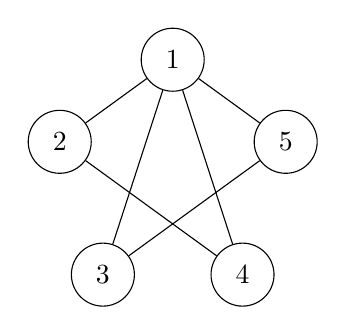
\begin{tikzpicture}[mystyle/.style={draw,circle,minimum size=8mm,inner sep=2pt}]
				\node[regular polygon,regular polygon sides=5,minimum size=3cm] (p) {};
				\foreach\x in {1,...,5}{\node[mystyle] (\x) at (p.corner \x){\x};}
				\draw  (1) -- (2);
				\draw  (1) -- (3);
				\draw  (1) -- (4);
				\draw  (1) -- (5);
				\draw  (2) -- (4);
				\draw  (3) -- (5);
				\end{tikzpicture}

			
			\end{figure}
			\end{center}
		\end{column}

		\begin{column}{.475\textwidth}
			\begin{center}
			\begin{figure}[H]
				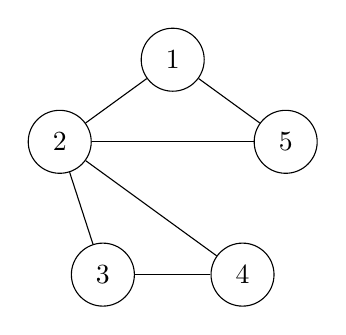
\begin{tikzpicture}[mystyle/.style={draw,circle,minimum size=8mm,inner sep=2pt}]
				\node[regular polygon,regular polygon sides=5,minimum size=3cm] (p) {};
				\foreach\x in {1,...,5}{\node[mystyle] (\x) at (p.corner \x){\x};}
				\draw  (1) -- (2);
				\draw  (1) -- (5);
				\draw  (2) -- (5);
				\draw  (2) -- (3);
				\draw  (2) -- (4);
				\draw  (3) -- (4);
				\end{tikzpicture}
			\end{figure}
			\end{center}
		\end{column}	
	\end{columns}
	\vspace{3px}
	Achtung: Die geometrische Anordnung auf dem Papier ist dabei irrelevant.
\end{frame}

\begin{frame}{Adjazenzmatrix}
	\begin{block}{Def.: Adjazenzmatrix}
		\begin{columns}
			\begin{column}{0.475\textwidth}
				Sei $G=(V_G,E_G)$ gerichteter Graph.\\
				Adjazenzmatrix $A \in \set{0,1}^{\mid V_G \mid \times \mid V_G \mid}$\\[12pt]
				\[
					A_{ij} = 
					\begin{cases}
						1, & \text{ falls } (i,j)\in E_G\\
						0, & \text{ falls } (i,j)\notin E_G
					\end{cases}
				\]
			\end{column}
			\begin{column}{0.475\textwidth}
				Sei $U=(V_U,E_U)$ ungerichteter Graph.\\
				Adjazenzmatrix $A \in \set{0,1}^{\mid V_U \mid \times \mid V_U \mid}$\\[12pt]
				\[
					A_{ij} = 
					\begin{cases}
						1, & \text{ falls } \set{i,j}\in E_U\\
						0, & \text{ falls } \set{i,j}\notin E_U
					\end{cases}
				\]
			\end{column}
		\end{columns}
	\end{block}
\end{frame}

\begin{frame}{Adjazenzmatrix}
	\begin{exampleblock}{Beispiele}
		\begin{columns}
			\begin{column}{0.475\textwidth}
				\begin{center}
					\begin{figure}[H]
				\begin{tikzpicture}[->,>=stealth,baseline=-5mm]
				\matrix[matrix of math nodes,nodes={draw,circle,minimum size=8mm,inner sep=2pt},row sep=10mm,column sep=10mm,ampersand replacement=\&]
				{
					|(0)| 0 \& |(1)| 1 \\
					|(2)| 2 \& |(3)| 3 \\
				};
				\draw  (0) -- (2);
				\draw  (0) edge [loop above] ();
				\draw  (1) -- (3);
				\draw  (2) to [bend right] (1);
				\draw  (1) to [bend right] (2);
				\end{tikzpicture}
				\end{figure}
				$\bordermatrix{
					  & 0 & 1 & 2 & 3 \cr
					0 & 1 & 0 & 1 & 0 \cr
					1 & 0 & 0 & 1 & 1 \cr
					2 & 0 & 1 & 0 & 0 \cr
					3 & 0 & 0 & 0 & 0 \cr
					}$
				\end{center}
			\end{column}
			\begin{column}{0.475\textwidth}
				\begin{center}
				\begin{figure}[H]
				\begin{tikzpicture}[>=stealth,baseline=-5mm, every loop/.style={}]
				\matrix[matrix of math nodes,nodes={draw,circle,minimum size=8mm,inner sep=2pt},row sep=10mm,column sep=10mm,ampersand replacement=\&]
				{
								\& |(1)| 1	\&  \\
					|(2)| 2 	\&			\& |(3)| 3  \\
				};
				\draw  (1) -- (2);
				\draw  (1) -- (3);
				\draw  (3) edge [loop right] ();
			\end{tikzpicture}
			\end{figure}
			$\bordermatrix{
					  & 0 & 1 & 2 & 3 \cr
					0 & 0 & 0 & 0 & 0 \cr
					1 & 0 & 0 & 1 & 1 \cr
					2 & 0 & 1 & 0 & 0 \cr
					3 & 0 & 1 & 0 & 1 \cr
					}$
			\end{center}
			\end{column}
		\end{columns}
	\end{exampleblock}
\end{frame}

\begin{frame}{Wegematrix}
	\begin{block}{Def.: Wegematrix}
		\begin{columns}
			\begin{column}{0.95\textwidth}
				Sei $G=(V_G,E_G)$ gerichteter Graph.\\
				Wegematrix $W \in \set{0,1}^{\mid V_G \mid \times \mid V_G \mid}$\\[12pt]
				\[
					W_{ij} = 
					\begin{cases}
						1, & \parbox[t]{.6\textwidth}{ falls es in $E_G$ Pfad von $i$ nach $j$ gibt.}\\
						0, & \parbox[t]{.6\textwidth}{ sonst}
					\end{cases}
				\]
			\end{column}
			% \begin{column}{0.475\textwidth}
			% 	Sei $U=(V_U,E_U)$ gerichteter Graph.\\
			% 	Wegematrix $W \in \set{0,1}^{\mid V_U \mid \times \mid V_U \mid}$\\[12pt]
			% 	\[
			% 		W_{ij} = 
			% 		\begin{cases}
			% 			1, & \parbox[t]{.6\textwidth}{ falls es in $E_U$ Pfad von $i$ nach $j$ gibt.}\\
			% 			0, & \parbox[t]{.6\textwidth}{ sonst}
			% 		\end{cases}
			% 	\]
			% \end{column}
		\end{columns}
	\end{block}
\end{frame}

\begin{frame}{Wegematrix}
	\begin{exampleblock}{Beispiele}
		\begin{columns}
			\begin{column}{0.95\textwidth}
				\begin{center}
					\begin{figure}[H]
				\begin{tikzpicture}[->,>=stealth,baseline=-5mm]
				\matrix[matrix of math nodes,nodes={draw,circle,minimum size=8mm,inner sep=2pt},row sep=10mm,column sep=10mm,ampersand replacement=\&]
				{
					|(0)| 0 \& |(1)| 1 \\
					|(2)| 2 \& |(3)| 3 \\
				};
				\draw  (0) -- (2);
				\draw  (0) edge [loop above] ();
				\draw  (1) -- (3);
				\draw  (2) to [bend right] (1);
				\draw  (1) to [bend right] (2);
				\end{tikzpicture}
				\end{figure}
				$\bordermatrix{
					  & 0 & 1 & 2 & 3 \cr
					0 & 1 & 1 & 1 & 1 \cr
					1 & 0 & 1 & 1 & 1 \cr
					2 & 0 & 1 & 1 & 1 \cr
					3 & 0 & 0 & 0 & 1 \cr
					}$
				\end{center}
			\end{column}
			% \begin{column}{0.475\textwidth}
			% 	\begin{center}
			% 	\begin{figure}[H]
			% 	\begin{tikzpicture}[>=stealth,baseline=-5mm, every loop/.style={}]
			% 	\matrix[matrix of math nodes,nodes={draw,circle,minimum size=8mm,inner sep=2pt},row sep=10mm,column sep=10mm,ampersand replacement=\&]
			% 	{
			% 					\& |(1)| 1	\&  \\
			% 		|(2)| 2 	\&			\& |(3)| 3  \\
			% 	};
			% 	\draw  (1) -- (2);
			% 	\draw  (1) -- (3);
			% 	\draw  (3) edge [loop right] ();
			% \end{tikzpicture}
			% \end{figure}
			% $\bordermatrix{
			% 		  & 0 & 1 & 2 & 3 \cr
			% 		0 & 1 & 1 & 1 & 0 \cr
			% 		1 & 1 & 1 & 1 & 0 \cr
			% 		2 & 1 & 1 & 1 & 0 \cr
			% 		3 & 1 & 1 & 1 & 0 \cr
			% 		}$
			% \end{center}
			% \end{column}
		\end{columns}
	\end{exampleblock}
\end{frame}